\subsection{Importing bitmap graph}
The simplest method to import get your Octave/Matlab graphs onto a document is to export them to a bitmap picture, and import like we did before.

Our code looks something like the following\footnotemark, and the full example is in \verb|Examples/Importing-graphs|.
\lstinputlisting[language=Matlab, caption={\texttt{Importing-graphs/bitmap/example.m}}]{Examples/Importing-graphs/bitmap/bitmap-code.m}
\footnotetext{You may notice the figure is exported to \texttt{.eps}, not \texttt{.png}, \texttt{.tiff} or something otherwise more common. For that you may want to look into \href{https://uk.mathworks.com/matlabcentral/fileexchange/23629-export_fig}{\texttt{export\_fig}}.}

Then, to include the graph, we simply use \verb|\includegraphics|.
\begin{lstlisting}
\begin{figure}[h]
    \centering
    \includegraphics[width=\textwidth]{figures/example.eps}
\end{figure}
\end{lstlisting}
Below you can see the output compared to something natively drawn with pgfplots.
It is a deliberately simple graph that can be easily replicated natively, but it highlights that font sizes and other small issues can become problematic for legibility.

\begin{figure}[h]
\centering
\begin{minipage}{0.50\textwidth}
    \includegraphics[width=\textwidth]{Examples/Importing-graphs/bitmap/figures/example.eps}
    \caption{Matlab}
\end{minipage}
\hfill
\begin{minipage}{0.48\textwidth}
    \begin{tikzpicture}[]
        \begin{axis}[xlabel= \( x \), ylabel = \( f(x) \) ]
            \addplot[domain=0:2*pi, samples=100, blue] {sin(deg(x))};
            \legend{ \( f(x) = \sin(x)  \) }
        \end{axis}
    \end{tikzpicture}
    \caption{Natively rendered}
\end{minipage}
\end{figure}

So what can we do instead? We can generate the graphs in Octave/Matlab and export the data for \texttt{tikz} and \texttt{pgfplots} to natively render it.
We have two options to do so: \texttt{matlab2tikz} and exporting to a \texttt{.svg} file.

\paragraph{Challenge:}
Replicate the sinusoidal graph with \texttt{pgfplots}, and you might see a straight line, indicating that it uses degrees, not radians.
Try to search for the solution!
Hopefully you will run into \href{https://tex.stackexchange.com/questions/16232/how-to-plot-fx-sinx-kx-cosx-and-ux-x%C2%B2-with-tikz}{this} link.

\subsection{Matlab2tikz}
This is an outstanding script written by Nico Schlömer which can be downloaded from Mathworks' \href{https://uk.mathworks.com/matlabcentral/fileexchange/22022-matlab2tikz-matlab2tikz}{file exchange}, or directly from the \href{https://github.com/matlab2tikz/matlab2tikz}{github}. Please refer to the installation on the github page, if you are unfamiliar with installing external matlab functions.
In short, use Set Path to include the downloaded \verb|src/| to your path.

Usage is very similar to exporting a bitmap image, the only difference is that we get a \texttt{.tex} to import, which can be further edited if you really want to:
\lstinputlisting[language=Matlab, caption={\texttt{Importing-graphs/matlab2tikz/mat2tikz.m}}]{Examples/Importing-graphs/matlab2tikz/mat2tikz.m}

Importing requires a few packages and settings, as can be seen below.
The information is extracted from \texttt{matlab2tikz}'s github, and reading their \href{https://github.com/matlab2tikz/matlab2tikz/wiki/FAQ}{FAQ} may be very helpful 

The code is not separated into preamble and content, but it should be clear what goes where.
Importantly, the whole example can be found in \texttt{Examples/Importing-graphs}.
\lstinputlisting[language=tex, caption={\texttt{Importing-graphs/matlab2tikz/totikz.tex}}]{Examples/Importing-graphs/matlab2tikz/totikz.tex}
Resulting in:
\begin{figure}[h]\centering
\begin{minipage}{0.49\textwidth}
    \newlength\fheight{} \newlength\fwidth{}
    \setlength\fheight{5.5cm}
    \setlength\fwidth{7cm}    
\input{Examples/Importing-graphs/matlab2tikz/figures/graph.tex}
\caption{Matlab generated and rendered natively}
\end{minipage}
\hfill
\begin{minipage}{0.49\textwidth}
    \begin{tikzpicture}[]
        \begin{axis}[xlabel= \( x \), ylabel = \( f(x) \),
            ymin=-1, xmin=0, ymax=1,]
            \addplot[domain=0:2*pi, samples=100, blue] {sin(deg(x))};
            \legend{ \( f(x) = \sin(x)  \) }
        \end{axis}
    \end{tikzpicture}
    \caption{Generated with pgfplots}
\end{minipage}
\end{figure}

Do you know why the fonts look still different? In the graph generated by matlab, we did not tell it to render using math mode --- f(x) vs \( f(x) \).

\subsection{Importing vector graph}